Den Zeeman-Effekt unterscheidet man durch seine \emph{normale} und \emph{anomale} Version, wobei erstere effektiv unter Spinvernachlässigung und letztere unter Spinberücksichtigung Aussagen über die Spektralaufspaltung trifft. Aus Sicht der klassischen Elektronenanschauung zerlegt man ein um den Atomkern oszillierendes Atom in drei Anschauungselektronen mit (i) linearer, (ii) positiver und (iii) negativer zirkularer Oszillation. Hierbei wird die Aufteilung unter Berücksichtigung des anliegenden linearen $B_0$ Feldes vorgenommen, wie Abbildung \ref{fig:ElektronenOszillationZerlegung} zeigt. 
\begin{figure}[H]
	\centering
	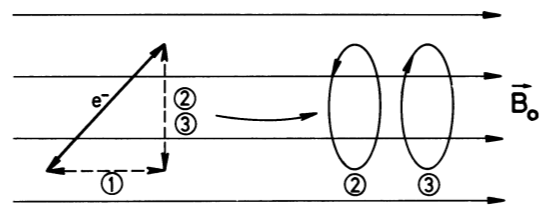
\includegraphics[width=5cm]{Bilddateien/Grundlagen/ElektronOszillationZerlegung.png}
	\caption{Zerlegung der Elektronenoszillation in drei Anschauungselektronen.}
	\label{fig:ElektronenOszillationZerlegung}
\end{figure}
Im Fall (i) finden wir $E\parallel B_0$ und keinerlei Frequenzänderung. Die Fälle (ii) und (iii) erfahren durch eine Änderung des Magnetfeldes jedoch mittels Induktion eine Beschleunigung, dessen Vorzeichen von der Umlaufrichtung abhängig ist. Der Betrag der Frequenzänderung ist dabei für $\mu_B$ als \emph{Bohrsches Magneton} gegeben durch 
\[
	\Delta\omega = \frac{\mu_B}{\hbar}\cdot\dabs{B_0}{}.
\]
Dies zeigt man im Wesentlichen durch Gleichsetzung der Coulomb- und Zentrifugalkräfte des Elektrons und kartesischer Zerlegung der so entstehenden Bewegungsgleichungen. Das entscheidende Ergebnis dieser Berechnungen ist jedoch der \emph{konstante} Aufspaltungsabstan einer Spektrallinie in drei äquidistante Linien, was durch dieses Modell beschrieben ist. Die Emissionsrichtung ist dabei durch die Magnetfeldrichtung gegeben \cite[p.216ff]{HakenWolf}.

\subsubsection*{Anomaler Zeeman Effekt}
	Beachtet man den Spin des Elektrons, so reicht das Modell des normalen Zeeman Effektes nicht mehr aus, denn eine eindeutige Beschreibung ist nur noch über die Quantenzahlen $S = \sum_{i\in I}s_i$ und $L = \sum_{i\in I}s_i$ mit $I$ Elektronenindexmenge möglich. Die Aufspaltung der Energieniveaus ist dann nicht mehr äquidistant, sondern wird durch die Landé-Faktorfunktion $g(J,L,S)$ beschrieben. Die Differenzenergie ist dann mit $m_J$ als Orientierungsquantenzahl des Gesamtdrehimpulses $J$ gegeben durch
	\[
		\Delta E = m_J\cdot g(J,L,S)\cdot\mu_B\cdot B_0.
	\]
	Der Aufspaltungsabstand ist daher direkt von $S$ und $L$ abhängig, wie die folgende Abbildung veranschaulicht \cite[p.219]{HakenWolf}.
	\begin{figure}[H]
		\centering
		\begin{subfigure}[b]{0.4\textwidth}
			\centering
			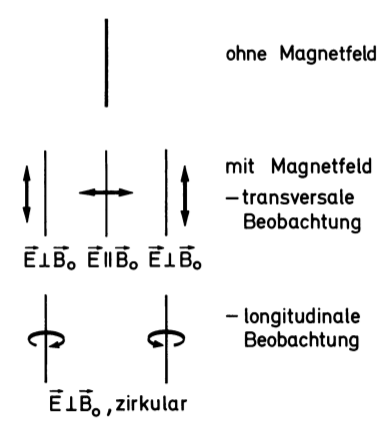
\includegraphics[height=5cm]{Bilddateien/Grundlagen/NormalZeemanAufspaltung.png}
			\caption{Normale Zeeman Aufspaltung.}
			\label{fig:NormalZeemanAufspaltung}
		\end{subfigure}
		\
		\begin{subfigure}[b]{0.4\textwidth}
			\centering
			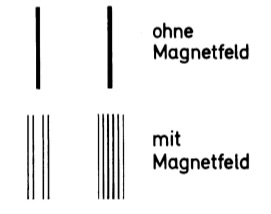
\includegraphics[height=5cm]{Bilddateien/Grundlagen/AnomalZeemanAufspaltung.png}
			\caption{Anomale Zeeman Aufspaltung.}
			\label{fig:AnomaleZeemanAufspaltung}
		\end{subfigure}
		\caption{Schematische Aufspaltung des normalen und anomalen Zeemaneffektes am Beispiel des (a) Cadamium und (b) Natrium.}
	\end{figure}
	In vektorieller Darstellung ist die Entstehung von $J$ durch die Kopplung von $L$ und $S$ gegeben. Ebenso koppeln die magnetischen Momente $\mu_L$ und $\mu_S$ zu $\mu_J$, dessen Richtung jedoch im Allgemeinen nicht mehr mit derjenigen von $J$ zusammenfällt (siehe Abbildung \ref{fig:VektormodellAnomalZeeman}). Projeziert man die Vektoren $J$ und $\mu_J$ jedoch auf eine Ebene, so lässt sich mittels Trigonometrie die Projektion von $\mu_J$ auf $J$ bzw schließlich auf das Magnetfeld $B$ durch den Landé-Faktor $g$ bestimmen (siehe Abbildung \ref{fig:ProjektionVektormodellAnomalerZeeman}) \cite[p.220]{HakenWolf}.
	\begin{figure}[H]
		\centering
		\begin{subfigure}[b]{0.4\textwidth}
			\centering
			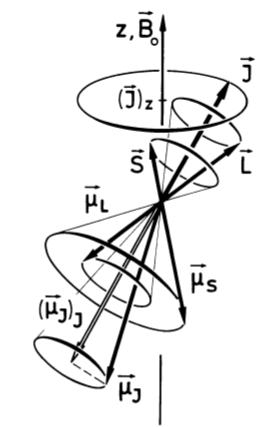
\includegraphics[height=5cm]{Bilddateien/Grundlagen/VektormodellAnomalZeeman.png}
			\caption{Vektormodell.}
			\label{fig:VektormodellAnomalZeeman}
		\end{subfigure}
		\
		\begin{subfigure}[b]{0.4\textwidth}
			\centering
			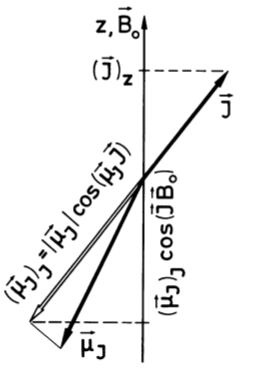
\includegraphics[height=5cm]{Bilddateien/Grundlagen/ProjektionVektormodellAnomalerZeeman.png}
			\caption{Projektion.}
			\label{fig:ProjektionVektormodellAnomalerZeeman}
		\end{subfigure}
		\caption{Vektormodell und Projektion des anomalen Zeeman Effektes.}
	\end{figure}

